\begin{figure}[ht!]
\centering
  \caption{Silhouette analysis}\label{fig:Silhouette}
   \begin{subfigure}[b]{\textwidth}
   \centering
   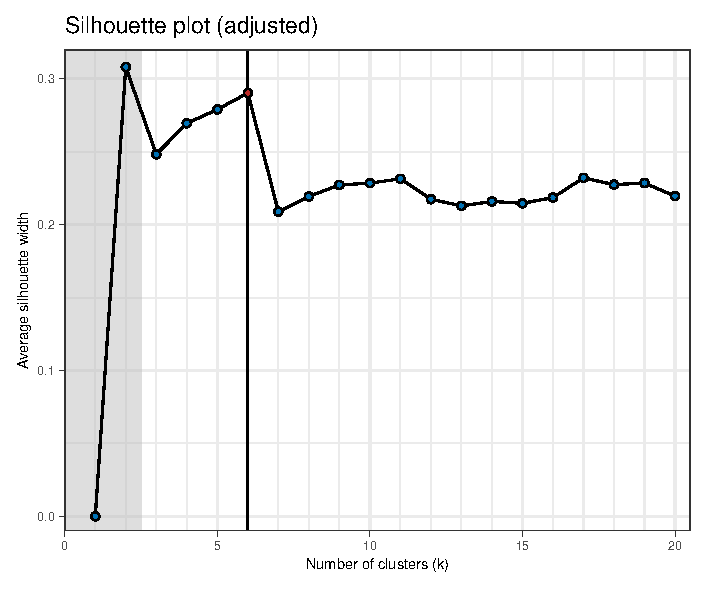
\includegraphics{Figures_Appendix/Figure_Silhouette_2.pdf}
   \caption{Average silhouette width for different numbers of clusters \textit{k}} \label{fig:G3_silhouette_2}
   \begin{subcaption2}
     This figure displays the average silhouette width across all clusters for different numbers of clusters \textit{k}. We perform k-means clustering on a dataset with 88 country-level observations. Observations include information on \textit{adjusted} feature importance, i.e., we adjust feature importance for country-level model performance. We also include information about the vertical distribution. Vertical line and red point indicate the number of clusters that maximizes average silhouette width across all number of clusters with $k>2$.
   \end{subcaption2}
   \end{subfigure}
 \end{figure}
 \clearpage

 \begin{figure}[ht!]\ContinuedFloat
   \centering
   \begin{subfigure}[b]{\textwidth}
   \centering
   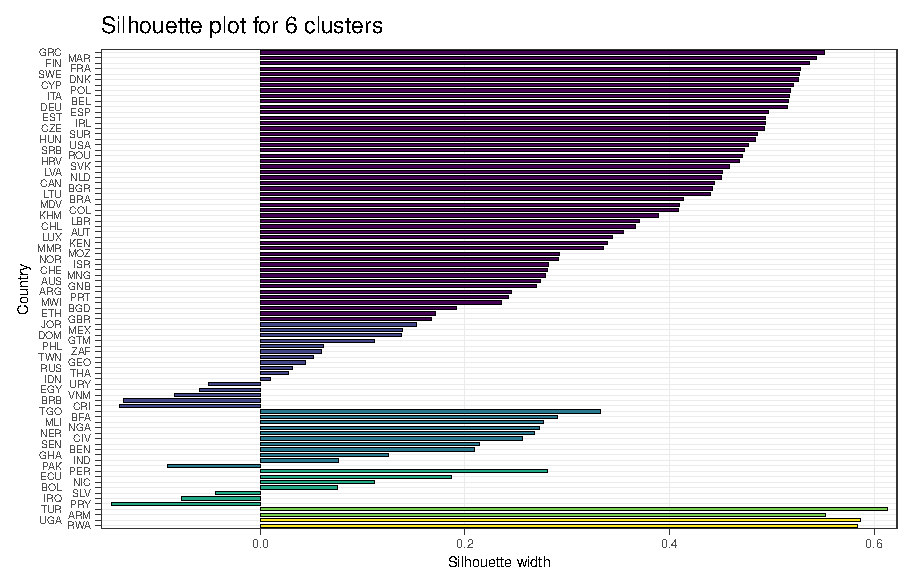
\includegraphics{Figures_Appendix/Figure_Silhouette_Clusters_2.pdf}
   \caption{Average silhouette width for each country per cluster \textit{k}} \label{fig:G4_silhouette_2}
   \begin{subcaption2}
     This figure displays the silhouette for each country for six clusters. We perform k-means clustering on a dataset with 88 country-level observations. Observations include information on \textit{adjusted} feature importance, i.e. we adjust feature importance for country-level model performance. We also include information about the vertical distribution. We order observations (y-axis) by clusters with most observations and by silhouette width. Silhouette width expresses how well each observation fits in its cluster, also in comparison to the observations from the least distant, but different cluster.
   \end{subcaption2}
   \end{subfigure}
 \end{figure}
 \clearpage

\begin{figure}[ht!]\ContinuedFloat
   \centering
   \begin{subfigure}[b]{\textwidth}
   \centering
   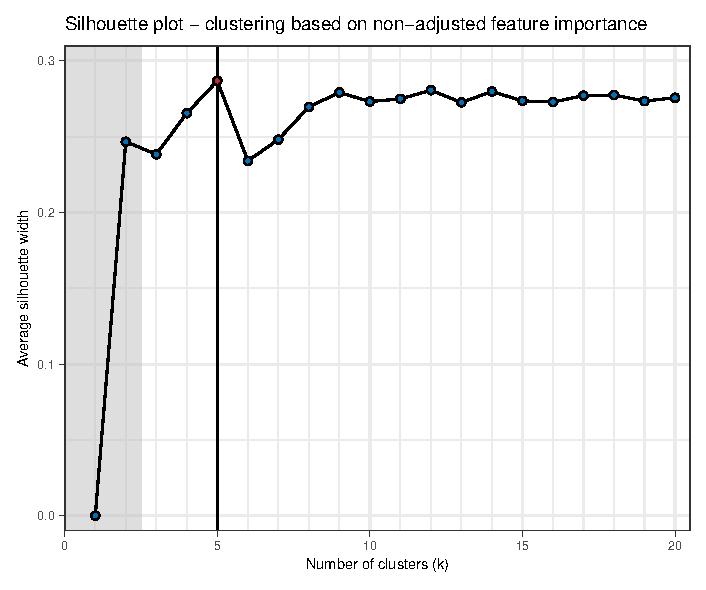
\includegraphics{Figures_Appendix/Figure_Silhouette_1.pdf}
   \caption{Average silhouette width for different numbers of clusters \textit{k}} \label{fig:G1_silhouette}
   \begin{subcaption2}
     This figure displays the average silhouette width across all clusters for different numbers of clusters \textit{k}. We perform k-means clustering on a dataset with 88 country-level observations. Observations include information on feature importance and the vertical distribution. In contrast to Figure \subref{fig:G3_silhouette_2}, we do not adjust feature importance for country-level model performance. Vertical line and red point indicate the number of clusters that maximizes average silhouette width across all clusters with $k>2$.
   \end{subcaption2}
   \end{subfigure}
 \end{figure}

 \clearpage

 \begin{figure}[ht!]\ContinuedFloat
   \centering
   \begin{subfigure}[b]{\textwidth}
   \centering
   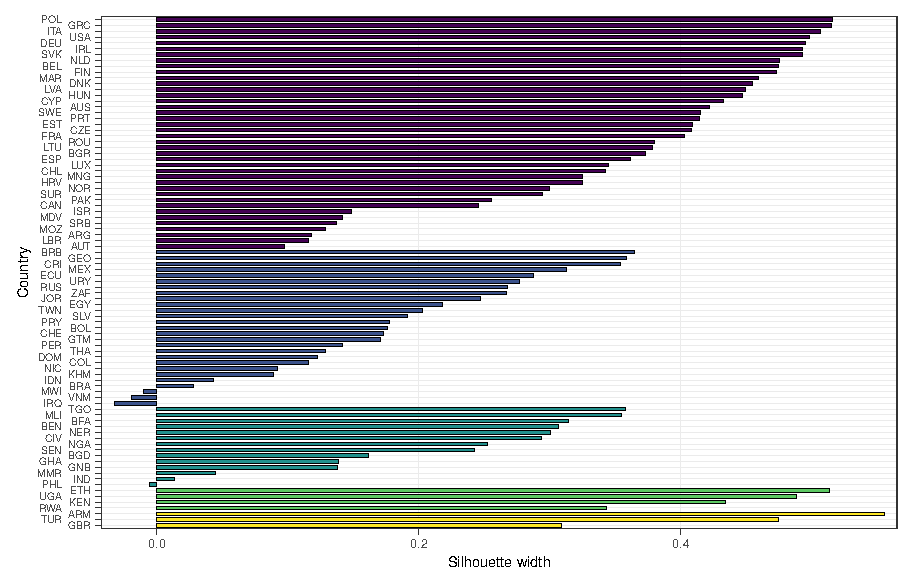
\includegraphics{Figures_Appendix/Figure_Silhouette_Clusters_1.pdf}
   \caption{Average silhouette width for each country per cluster \textit{k}} \label{fig:G2_silhouette}
   \begin{subcaption2}
     This figure displays the silhouette for each country for 11 clusters. We perform k-means clustering on a dataset with 88 country-level observations. Observations include information on feature importance and the vertical distribution. In contrast to Figure \subref{fig:G2_silhouette}, we do not adjust feature importance for country-level model performance. We order observations (y-axis) by clusters with most observations and by silhouette width. Silhouette width expresses how well each observation fits in its cluster, also in comparison to the observations from the least distant, but different cluster.
   \end{subcaption2}
   \end{subfigure}
 \end{figure}
 \clearpage

 \begin{figure}[ht!]\ContinuedFloat
   \centering
   \begin{subfigure}[b]{\textwidth}
   \centering
   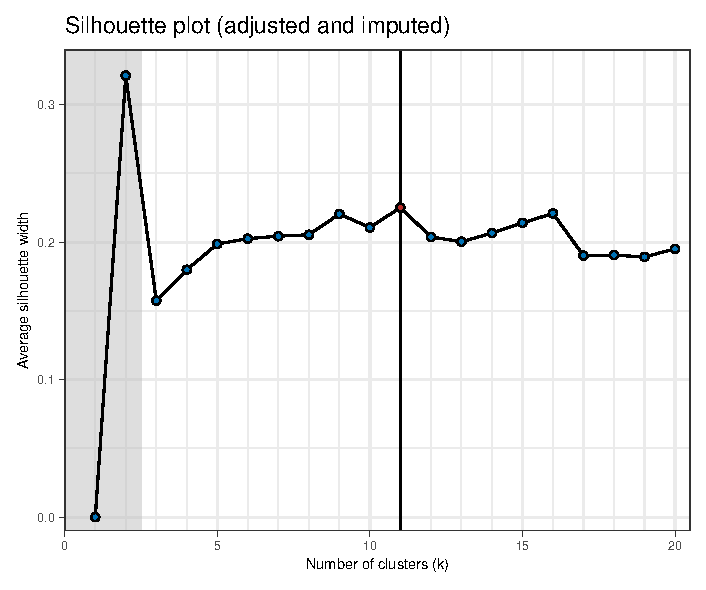
\includegraphics{Figures_Appendix/Figure_Silhouette_3.pdf}
   \caption{Average silhouette width for different numbers of clusters \textit{k}} \label{fig:G1_silhouette_3}
   \begin{subcaption2}
     This figure displays the average silhouette width across all clusters for different numbers of clusters \textit{k}. We perform k-means clustering on a dataset with 88 country-level observations. Observations include information on feature importance and the vertical distribution. In contrast to Figure \subref{fig:G3_silhouette_2}, we impute missing values for unobserved features with the average feature importance for each feature. We adjust feature importance for country-level model performance. Vertical line and red point indicate the number of clusters that maximizes average silhouette width across all clusters with $k>2$.
   \end{subcaption2}
   \end{subfigure}
 \end{figure}

 \clearpage

 \begin{figure}[ht!]\ContinuedFloat
   \centering
   \begin{subfigure}[b]{\textwidth}
   \centering
   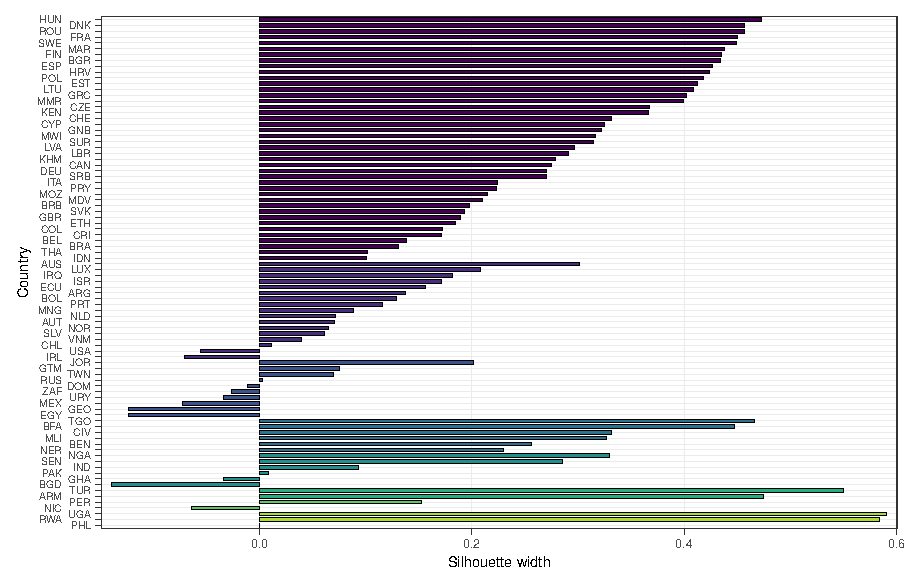
\includegraphics{Figures_Appendix/Figure_Silhouette_Clusters_3.pdf}
   \caption{Average silhouette width for each country per cluster \textit{k}} \label{fig:G2_silhouette_3}
   \begin{subcaption2}
     This figure displays the silhouette for each country for 11 clusters. We perform k-means clustering on a dataset with 88 country-level observations. Observations include information feature importance and the vertical distribution. In contrast to Figure \subref{fig:G2_silhouette}, we impute missing values for unobserved features with the average feature importance for each feature. We adjust feature importance for country-level model performance.  We order observations (y-axis) by clusters with most observations and by silhouette width. Silhouette width expresses how well each observation fits in its cluster, also in comparison to the observations from the least distant, but different cluster.
   \end{subcaption2}
   \end{subfigure}
 \end{figure}
 \clearpage